
%============================================================
\subsection{\texttt{ell\_shape}}
\label{subsec:geometry_ell_shape}
%============================================================

\noindent
\textbf{Geometry ID:} \texttt{GLOB-GEO0006}
\qquad
\textbf{Version:} \texttt{1.0.0}

\begin{figure}[htbp]
    \centering
    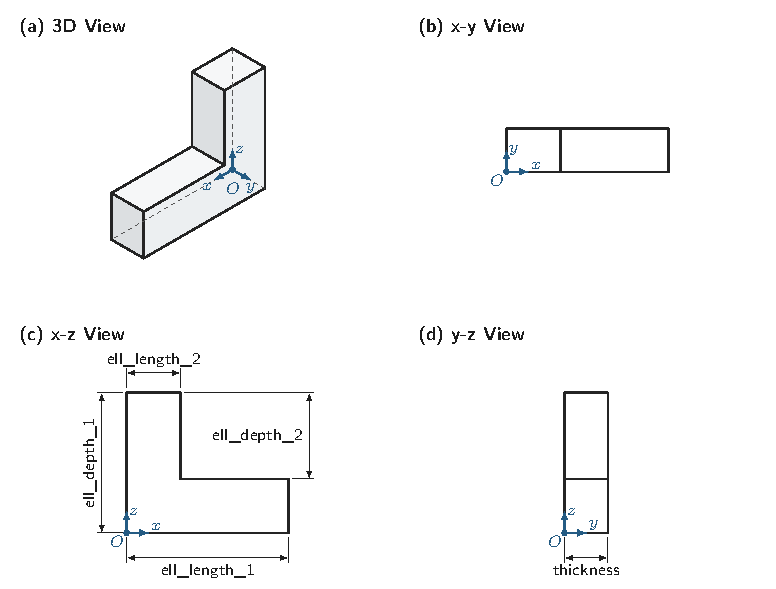
\includegraphics[width=0.65\linewidth]
    {./figs/geometries/ell_shape.pdf}
    \caption{Standardized parametrization and local
    coordinate system of the L-shaped geometry.}
    \label{fig:ell_shape}
\end{figure}

The \texttt{ell\_shape} geometry represents an
L-shaped specimen formed by two orthogonal legs
with uniform thickness.

As illustrated in Fig.~\ref{fig:ell_shape},
the local coordinate system is defined by
the right-handed Cartesian axes $x$, $y$,
and $z$. The origin $O$ is located at the
exterior corner of the L-shaped profile on
the reference face $y=0$, corresponding to
$x=0$ and $z=0$.

The positive $x$ and $z$ directions extend
from the origin into the specimen along
its overall length and depth, respectively.
The $y$ axis represents the thickness direction.

The L-shaped profile lies in the local
$x$--$z$ plane and is extruded along the
positive $y$ direction.

\paragraph{Independent parameters.}

The geometry is defined by five required
parameters, all expressed in millimeters:

\begin{itemize}
    \item \texttt{thickness}: uniform specimen
    thickness along the local $y$ axis;

    \item \texttt{ell\_length\_1}: overall
    specimen dimension along the local $x$ axis;

    \item \texttt{ell\_depth\_1}: overall
    specimen dimension along the local $z$ axis;

    \item \texttt{ell\_length\_2}: width along
    the local $x$ direction of the leg extending
    through the full specimen depth;

    \item \texttt{ell\_depth\_2}: distance along
    the local $z$ direction from the reentrant
    corner to the end of the full-depth leg.
\end{itemize}

The reentrant corner of the L-shaped profile
is located at

\begin{equation}
\begin{aligned}
x &= \texttt{ell\_length\_2},\\
z &= \texttt{ell\_depth\_1}
     -\texttt{ell\_depth\_2}.
\end{aligned}
\end{equation}

\paragraph{Geometric constraints.}

All five parameters must be strictly positive.
The dimensions must additionally satisfy

\begin{align}
\texttt{ell\_length\_2}
&< \texttt{ell\_length\_1},
\\
\texttt{ell\_depth\_2}
&< \texttt{ell\_depth\_1}.
\end{align}

These conditions ensure that both orthogonal
legs have positive dimensions and that
the L-shaped profile contains a well-defined
reentrant corner.
